\section{Second-order theory of the ring}\label{sec:ring}

\paragraph{In brief.}
For a rare parasite, the second-order growth loss is the leading effect of small host fluctuations. When scarcity wastes failed transfers, stays are memoryless, and independent hosts have nonnegative memory, a sufficiently long steady stay reduces this loss at fixed existing stays. Obligate host count alone provides no protection. At fixed mean total transfer, independent alternative hosts with matched fluctuation laws reduce that transfer's contribution to the loss.

Host fluctuations affect a parasite through the times at which its descendants encounter each host. We analyze this sampling to second order in the gain-only ring of Section~\ref{sec:model}, with arithmetic-mean rates as baseline and $\sigma^2 > 0$ for strict comparisons. Write $C$ for the coefficient of per-step growth cost $\ln\lambda-r$ and $\Gamma = \mathcal{T} C \sigma^2$ for the loss per lineage generation. Proofs are in Appendix~\ref{app:ring}, and verification details are in Online Resource~1.

\subsection{Returns of a line of descent and the ring formula}\label{subsec:ring-formula}

The second-order cost can be written in terms of the time between successive uses of a transfer by a reference lineage (the renewal gap $L_e$, of mean $\mathcal{T}_e$; Proposition~\ref{prop:ring-lineage}, Appendix~\ref{app:ring}).

The ring is primitive when $n = 1$ or some $s_k > 0$. Stage $k$ has lineage staying probability $m_k = s_k / \lambda < 1$. Its geometric stay on $\{1, 2, \dots\}$ has mean $\tau_k = 1/(1 - m_k) \ge 1$, and $\mathcal{T} = \sum_{k=1}^n \tau_k$. One circuit separates successive uses of a transfer.

\begin{proposition}[One fluctuating transfer in a geometric ring]\label{prop:ring-gamma}
In a primitive $n$-stage gain-only ring with fixed stays $s_k \ge 0$, mean transfers $g_k > 0$, lineage stays $\tau_k = 1/(1 - s_k/\lambda)$, and generation time $\mathcal{T} = \sum_{k=1}^n \tau_k$, let one transfer carry $h(t) = \exp(z(t) - \sigma^2/2)$ with centered stationary Gaussian $\mathrm{AR}(1)$ driver $z(t)$ of variance $\sigma^2 > 0$ and autocorrelation $\phi^\ell$ ($0 \le \phi < 1$), while all other entries are fixed. Put $\theta = \phi/(1 - \phi)$ and $R = \prod_{k=1}^n (1 + \tau_k/\theta)^{-1}$ for $\phi > 0$ ($R = 0$ at $\phi = 0$). Then $C = (1 + 2\theta)/(2\mathcal{T}^2) - \mathcal{T}^{-1} R/(1 - R)$, and the second-order loss per generation is
\begin{equation}
\Gamma = \sigma^2 \left[ \frac{1 + 2\theta}{2\mathcal{T}} - \frac{R}{1 - R} \right].
\label{eq:ring-gamma}
\end{equation}
Neither which transfer fluctuates nor the cyclic order of stages changes $\Gamma$. Independent $\mathrm{AR}(1)$ hosts add their coefficients, and for each fixed primitive ring of this form $\ln\lambda - r = C\sigma^2 + O(\sigma^4)$ as $\sigma \to 0$ (Theorem~\ref{thm:ring-rem-ar1}).
\end{proposition}

Equation~\eqref{eq:ring-gamma} separates two opposing effects of positive host memory, namely integrated host variance $(1 + 2\theta)/(2\mathcal{T})$ and the return discount $R/(1 - R)$ across circuits.

\subsection{The band and comparisons across hosts in series}\label{subsec:ring-series}

Bounds on $R$ confine $\Gamma$ to a band.

\begin{proposition}[The band, memory limits, and unequal stays]\label{prop:ring-band}
Under Proposition~\ref{prop:ring-gamma} ($0 \le \phi < 1$, $\sigma^2 > 0$),
\begin{equation}
\frac{\sigma^2}{2\mathcal{T}} \le \Gamma \le \frac{\sigma^2(1 + 2\theta)}{2\mathcal{T}},
\label{eq:ring-band}
\end{equation}
with left equality if and only if $\phi = 0$ or $n = 1$, so $\phi > 0$ strictly raises $\Gamma$ when $n \ge 2$. As $\phi \to 0$, $C \to 1/(2\mathcal{T}^2)$. Taking $C$ first and then $\phi \uparrow 1$, $C \to (1 - \mathrm{CV}^2)/(2\mathcal{T})$, where $\mathrm{CV}^2 = \Var(L)/\mathcal{T}^2$ and $\Var(L) = \sum_{k=1}^n \tau_k(\tau_k - 1)$. At fixed $n$, $\mathcal{T}$, and $0 < \phi < 1$, equal stays maximize $\Gamma$ and setting $n - 1$ stays to $1$ minimizes it (all tie at $\phi = 0$).
\end{proposition}

Two stays long relative to $\theta$ can approach the upper edge. One long stay does not suffice (details in Online Resource~1).

The effect of sequential hosts depends on what is held fixed.

\begin{proposition}[Hosts in series]\label{prop:ring-series}
Let all $n$ transfers of a primitive gain-only ring follow independent Gaussian $\mathrm{AR}(1)$ hosts with variance $\sigma^2 > 0$ and memory $0 \le \phi < 1$. Put $\bar{\tau} = \mathcal{T}/n$ and $P = \prod_{k=1}^n (1 + \tau_k/\theta)$ for $\phi > 0$.
\begin{enumerate}
\item[(i)] At fixed $\bar{\tau}$, $\sigma^2/(2\bar{\tau}) \le \Gamma \le \sigma^2(1 + 2\theta)/(2\bar{\tau})$, with left equality if and only if $\phi = 0$ or $n = 1$; no ring beats one stage at $\bar{\tau}$, though $n$ does not order $n \ge 2$ (at $\phi = 0.9$, stays $(10, 10)$ give $0.371\sigma^2$ whereas $(1, 1, 28)$ give $0.214\sigma^2$).
\item[(ii)] For equal stays $\tau$ and $a = 1 + \tau/\theta$, $\Gamma_n = \sigma^2[(1 + 2\theta)/(2\tau) - n/(a^n - 1)]$ ($\phi > 0$), strictly increasing in $n$ at fixed $\tau$ and strictly decreasing in $\tau$ at fixed $n$ ($\sigma^2/(2\tau)$ at $\phi = 0$).
\item[(iii)] Keeping existing $\tau_k$ fixed and appending a stage of stay $\mathcal{T}/n$ on its own host changes $\Gamma$ by $\sigma^2[P(x - 1) + 1]/[(P - 1)\{P(1 + x/n) - 1\}]$ ($x = \mathcal{T}/\theta$), positive for $0 < \phi < 1$ and zero at $\phi = 0$ (fixing physical rates instead alters $\lambda$ and every $\tau_k$).
\item[(iv)] Multiplying every $\tau_k$ by $c > 1$ at fixed host laws strictly lowers $\Gamma$.
\item[(v)] At fixed equal rates ($\tau > 1$, $0 < \phi < 1$), the per-step coefficient $f_n = (1 + 2\theta)/(2n\tau^2) - [\tau(a^n - 1)]^{-1}$ has increments $f_{n+1} - f_n$ changing sign at most once, and some $f_n > f_1$ if and only if $\theta > \tau/[2(\tau - 1)]$.
\end{enumerate}
\end{proposition}

\subsection{A steady stage and alternative hosts}\label{subsec:ring-steady}

We test Dobson's storage (``parking lot'') argument \citep{dobson2020} by adding a steady stage at fixed existing geometric lineage stays and host laws.

\begin{proposition}[Adding a steady stage and the diffusion index]\label{prop:ring-steady}
For independent $\mathrm{AR}(1)$ hosts ($0 \le \phi_k < 1$) in a primitive geometric ring, put $S_I = \sum_{k=1}^n \sigma_k^2(1 + 2\theta_k)$, $S = \sum_{k=1}^n \sigma_k^2$, and second-order per-step growth-variance term $V = S_I / \mathcal{T}^2$.
\begin{enumerate}
\item[(a)] Adding stay $t$ with host variance $v$ and memory $\theta_v$ lowers $\mathcal{T}V = S_I / \mathcal{T}$ if and only if $v(1 + 2\theta_v)/t < S_I / \mathcal{T}$; a steady stage ($v = 0$) lowers $\mathcal{T}V$ whenever $S_I > 0$ (leaving zero unchanged).
\item[(b)] When all $\phi_k = 0$, $\Gamma = S/(2\mathcal{T})$ changes by $(v\mathcal{T} - St)/[2\mathcal{T}(\mathcal{T} + t)]$, negative if and only if $v/t < S/\mathcal{T}$.
\item[(c)] For one fluctuating host of stay $a \ge 1$ ($\sigma^2 > 0$, $0 \le \phi < 1$) and one steady stage of stay $b \ge 1$ (not both $1$), against $\Gamma(a)/\sigma^2 = 1/(2a)$ for one stage,
\begin{equation}
\frac{\Gamma(a,b)}{\sigma^2} = \frac{1 + 2\theta}{2(a + b)} - \frac{\theta^2}{\theta(a + b) + ab}, \qquad \lim_{b \to \infty} \frac{(a + b)\Gamma(a,b)}{\sigma^2} = \frac{1 + 2\theta}{2} - \frac{\theta^2}{\theta + a},
\label{eq:ring-steady}
\end{equation}
so $\Gamma(a,b) \to 0$ as $b \to \infty$ at fixed $a, \theta$ (taking $\sigma \to 0$ before $b \to \infty$).
\item[(d)] With one fluctuating host ($\sigma^2 > 0$, $0 \le \phi < 1$), put $k = 2\Gamma/(\mathcal{T}V) \in [1/(1 + 2\theta), 1]$, $L = \ln R_0 / \sigma^2$, and $E = 2(\ln R_0 - \Gamma)/(\mathcal{T}V) = 2\mathcal{T}\ln R_0 / [\sigma^2(1 + 2\theta)] - k$. In a Brownian diffusion with drift $\mu = \ln R_0 - \Gamma > 0$ and variance rate $\mathcal{T}V$, the ever-fall probability by log size $x > 0$ is $\exp(-Ex)$ (and equals one if $\mu \le 0$). At fixed $a$, host law, and $\ln R_0$,
\begin{equation}
E(a,b) - E(a) = \frac{2b}{1 + 2\theta}\left[ L - \frac{a\theta}{a\theta + b(a + \theta)} \right],
\label{eq:ring-index-diff}
\end{equation}
positive for $b > b_* = [a\theta/(a + \theta)](1 - L)/L$ when $0 < L < 1$, positive for all $b > 0$ when $L \ge 1$, and negative when $L<0$ or when $L=0$ and $\theta>0$ (zero when $L=\theta=0$) ($\Delta\ln R_0 > \theta\sigma^2$ suffices for any added stay $\Delta$ to raise $E$).
\end{enumerate}
\end{proposition}

\begin{figure}
\centering
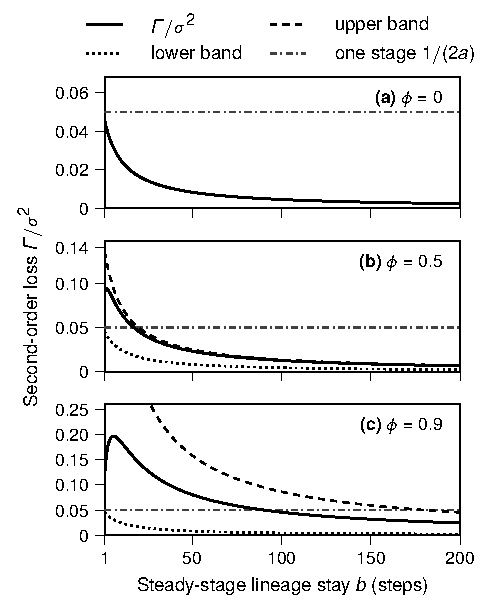
\includegraphics[width=84mm]{figures/ring-1.pdf}
\caption{Second-order loss per generation per unit log-host variance, $\Gamma/\sigma^2$, against steady stay $b$ with illustrative fluctuating stay $a = 10$: (a) $\phi = 0$, (b) $\phi = 0.5$, (c) $\phi = 0.9$. Solid curves: Eq.~\eqref{eq:ring-steady}; dotted and dashed curves: lower and upper edges of Eq.~\eqref{eq:ring-band}; dash-dotted lines: one-stage value $1/(2a) = 0.05$. Both edges coincide with the closed form at $\phi = 0$}
\label{fig:ring-1}
\end{figure}

With positive memory, a short steady stage can raise $\Gamma$ above $1/(2a)$ before longer stays send it to zero (Fig.~\ref{fig:ring-1}). The index $E$ describes infinite-horizon Brownian diffusion, not matrix first passage. Its crossing $b_*$ can differ from finite-horizon crossings, and $b_* \to \infty$ as $L \to 0^+$ at fixed $\theta, \sigma^2 > 0$. Worked examples and simulation details are in Online Resource~1.

Parallel alternative hosts at one transfer enter with squared shares \citep{doak1998}. Fluctuating staying can instead yield a gain.

\begin{proposition}[Alternative hosts at one step and fluctuating staying]\label{prop:ring-alt}
Replacing one transfer multiplier of the primitive gain-only ring by $\sum_{m=1}^M \pi_m h_m(t)$ ($\pi_m \ge 0$, $\sum_{m=1}^M \pi_m = 1$) at fixed mean total transfer and independent $\mathrm{AR}(1)$ hosts ($\sigma_m^2$, $0 \le \phi_m < 1$) gives
\begin{equation}
\Gamma_{\mathrm{alt}} = \sum_{m=1}^M \pi_m^2 \sigma_m^2 \left[ \frac{1 + 2\theta_m}{2\mathcal{T}} - \frac{R_m}{1 - R_m} \right], \qquad R_m = \prod_{k=1}^n \frac{1}{1 + \tau_k/\theta_m} \quad (R_m = 0 \text{ at } \phi_m = 0),
\label{eq:ring-alt}
\end{equation}
with per-step remainder $O(\sigma^4)$ along a fixed noise direction (Theorem~\ref{thm:ring-rem-ar1}). Equal shares of $M$ independent equal-variance, equal-memory hosts divide that step's coefficient by $M$, whereas equal shares of variances $\sigma^2$ and $9\sigma^2$ with the original memory multiply it by $2.5$ (and correlated hosts yield the factor $[1 + \rho(M - 1)]/M$ only under equal shares, equal variances, and cross-covariances equal to $\rho$ times the common autocovariance). Conversely, multiplying a positive staying contribution ($m_k > 0$) by a lognormal $\mathrm{AR}(1)$ factor ($\varsigma^2 > 0$, $0 \le \psi < 1$) at fixed transfers gives per-step cost $\varsigma^2[e_k^2(1 + 2\theta)/2 - e_k\psi m_k / \{(1 - \psi m_k)(1 - R)\}]$ ($e_k = (\tau_k - 1)/\mathcal{T}$; $\theta, R$ at $\psi$), which is negative when $\psi m_k / [(1 - \psi m_k)(1 - R)] > e_k(1 + 2\theta)/2$.
\end{proposition}

\begin{remark}\label{rem:ring-joint-stay}
When transfer into and staying inside a host of stay $b$ are driven jointly by one $\mathrm{AR}(1)$ innovation as in Appendix~\ref{app:ring} (reproduced independently), the coefficient grows as $\kappa^2(1 - \phi^2)b/2$ as $b \to \infty$ without being monotone or bounding bounded-probability host mortality.
\end{remark}

\subsection{Cyclic and periodic hosts, and continuous time}\label{subsec:ring-cyclic}

For cyclic or seasonal hosts, the host spectral density weights a demographic frequency-response function $K(\omega)$ \citep{tuljapurkar1985,bacaer2007}.

\begin{proposition}[Quasi-cycles and spectral response]\label{prop:ring-spectrum}
For one unit-sensitivity transition of a finite primitive model with renewal gap $L_e$ of mean $\mathcal{T}_e = \E[L_e]$:
\begin{enumerate}
\item[(a)] If the autocorrelation is the finite real-valued mixture $\rho(\ell) = \sum_{j=1}^{J} B_j z_j^\ell$ ($\ell \ge 1$, $|z_j| < 1$), $C = S_0/(2\mathcal{T}_e^2) - \mathcal{T}_e^{-1}\sum_j B_j R_e(z_j)/[1 - R_e(z_j)]$ with $S_0 = 1 + 2\sum_j B_j z_j/(1 - z_j)$ and $R_e(z) = \E[z^{L_e}]$ (specializing to $X_t = 2r_c\cos\omega_0\,X_{t-1} - r_c^2 X_{t-2} + \text{noise}$, $0 < r_c < 1$, $0 < \omega_0 < \pi$, via $z = r_c\ee^{\mathrm{i}\omega_0}$, $\rho(1) = 2r_c\cos\omega_0/(1 + r_c^2)$, $B = 1 + \mathrm{i}[\cos\omega_0 - \rho(1)/r_c]/\sin\omega_0$, and weights $B/2, \bar{B}/2$).
\item[(b)] If the driver has spectral density $f(\omega)$ on $(0,\pi)$ with $\pi^{-1}\int_0^\pi f(\omega)\dd\omega = 1$, put $g(\omega) = \E[\ee^{\mathrm{i}\omega L_e}]$. Then
\begin{equation}
C = \frac{1}{\pi}\int_0^\pi f(\omega) K(\omega)\dd\omega, \qquad K(\omega) = -\frac{1}{\mathcal{T}_e}\operatorname{Re}\frac{g(\omega)}{1 - g(\omega)}.
\label{eq:ring-spectrum}
\end{equation}
\item[(c)] On $(0,\pi)$, $K(\omega)$ has mean $1/(2\mathcal{T}_e^2)$ and limit $\lim_{\omega \to 0} K(\omega) = (1 - \mathrm{CV}^2)/(2\mathcal{T}_e)$ ($\mathrm{CV}^2 = \Var(L_e)/\mathcal{T}_e^2$). For one-stage transfer $K(\omega) = 1/(2\tau^2)$ is constant; for $n \ge 2$ in a primitive ring $\lim_{\omega \to 0} K(\omega) > 1/(2\mathcal{T}_e^2)$; $K(\omega) < 0$ if and only if $\operatorname{Re} g(\omega) > |g(\omega)|^2$; and $K(\omega)$ need not be monotone in $\omega$.
\end{enumerate}
\end{proposition}

\begin{figure}
\centering
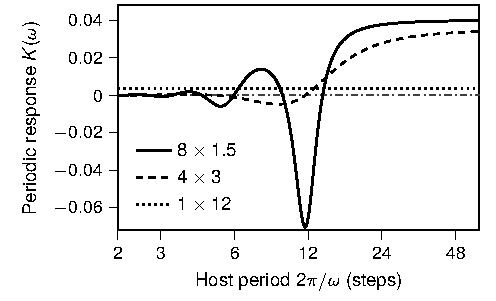
\includegraphics[width=84mm]{figures/ring-2.pdf}
\caption{Periodic response $K(\omega)$ against host period $2\pi/\omega$ (steps), from Eq.~\eqref{eq:ring-spectrum}, for illustrative primitive rings with $\mathcal{T} = 12$ steps. Stays: eight of $1.5$ (solid), four of $3$ (dashed), and one of $12$ (dotted, also the frequency average $1/(2\mathcal{T}^2) \approx 0.00347$). Thin dash-dotted line: $K = 0$}
\label{fig:ring-2}
\end{figure}

Formally, a sinusoidal multiplier $1 + \epsilon\cos(\omega t)$ ($|\epsilon| < 1$, $\omega \notin \pi\mathbb{Z}$) changes growth by $-(\epsilon^2/2)K(\omega)$ to second order ($\epsilon^2$ at period two, with a possible cubic term at period three). Concentrating circuit times around the host period can give $K(\omega) < 0$ (Fig.~\ref{fig:ring-2}). Numerical examples and the $\mathrm{AR}(2)$ check are in Online Resource~1.

In continuous time, a single fluctuating transfer has no cost in a one-stage cycle, while longer cycles retain a second-order cost (Proposition~\ref{prop:ring-ct}, Appendix~\ref{app:ring}).

Here ``one stage'' means one differential equation. No remainder bound is proved for this continuous-time lognormal family (example in Online Resource~1).

\subsection{Remainder theorems}\label{subsec:ring-remainder}

Bounded-perturbation analyticity \citep{ruelle1979}, independent invertible-matrix theorems \citep{lepage1989,hennion1991}, and compact-environment results \citep{steinsaltz2011} omit correlated lognormal multipliers on possibly singular primitive matrices. Reproductive-value normalization \citep{engen2013} gives fourth-order bounds in discrete time.

For a fixed primitive ring with Gaussian autoregressive hosts and sufficiently small noise, the error after the quadratic term is bounded by a constant times the fourth power of noise amplitude (Theorem~\ref{thm:ring-rem-ar1}, Appendix~\ref{app:ring}). The same error bound holds uniformly on compact families of primitive mean matrices (Lemma~\ref{lem:ring-rem-uniform}, Appendix~\ref{app:ring}). It also covers Gaussian linear processes built from absolutely summable weights on past innovations, including linked drivers (Theorem~\ref{thm:ring-rem-lin}, Appendix~\ref{app:ring}).

These bounds yield no usable numerical constants and no uniform control near non-primitivity, closing spectral gaps, host autocorrelations approaching $\pm1$, or growing $n$, nor was Lemma~\ref{lem:ring-rem-uniform} extended to general linear processes.

\subsection{Density dependence in transfers and the \texorpdfstring{$n$}{n}th root}\label{subsec:ring-density}

We test whether counting every transfer as a birth ($R_0^{1/n}$) calms endemic dynamics \citep{dobson2020} in a deterministic constant-host ring with donor-stage transfer regulation.

\begin{proposition}[Deterministic regulated loop]\label{prop:ring-reg}
In $\dd x_{k+1}/\dd t = c_k f_k(x_k) x_k - a_{k+1} x_{k+1}$ ($k$ modulo $n$, $c_k, a_k > 0$, $R_0 = \prod_{k=1}^n (c_k / a_k) > 1$), let each $f_k$ be differentiable, positive, nonincreasing, with $f_k(0) = 1$. Assume an equilibrium $\mathbf{x}^* > \mathbf{0}$ exists, and set $\kappa_k = -x_k^* f_k'(x_k^*)/f_k(x_k^*) \ge 0$ and $G = \prod_{k=1}^n (1 - \kappa_k)$.
\begin{enumerate}
\item[(a)] Eigenvalues at $\mathbf{x}^*$ solve $\prod_{k=1}^n (z + a_k) = G\prod_{k=1}^n a_k$; if $|G| < 1$, $\mathbf{x}^*$ is locally asymptotically stable for all $a_k > 0$.
\item[(b)] At equal exit rates $a_k = a = n/\tau$, eigenvalues are $a(\zeta - 1)$ ($\zeta^n = G$), giving return rate $a(1 - G^{1/n})$ for $0 < G < 1$, instability for $G > 1$, and for $G < 0$ stability when $n = 1, 2$ or $|G| < \sec^n(\pi/n)$ ($n \ge 3$) and instability when $|G| > \sec^n(\pi/n)$ \citep{tyson1978,thron1991,arcak2006}.
\item[(c)] Under $a_k = n/\tau$, $f(x) = \ee^{-x/K}$ in one transfer gives $G = 1 - \ln R_0$, stable for all $R_0 > 1$ at $n = 1, 2$ and critical $\ln R_0 = 1 + \sec^n(\pi/n)$ at $n \ge 3$ ($9, 5, 3.885$ for $n = 3, 4, 5$, approaching $2$). With $\ee^{-x_k/K}$ in every transfer and equal $a, c, K$ at $x_k^* = K\ln R_0 / n$ ($s = \ln R_0 / n$), return rate is $\ln R_0 / \tau$ for $s \le 1$, and critical $\ln R_0$ is $2n$ (even $n$) or $n[1 + \sec(\pi/n)]$ (odd $n \ge 3$), exceeding the one-transfer threshold for all $n \ge 4$ \citep{smith1987,muller2006,strelkowa2010}; for even $n$, alternating equilibria $s \pm d$ ($d = s\tanh(d/2) > 0$) are locally stable just above $s = 2$.
\item[(d)] Renaming $R_0$ as $R_0^{1/m}$ by counting $m$ births alters no stability threshold.
\end{enumerate}
\end{proposition}

\begin{remark}\label{rem:ring-reg-odd}
Equal exit rates are essential in part~(c). For odd $n \ge 3$ under shared exponential regulation, a simple pair crosses transversely at $s = 1 + \sec(\pi/n)$ with negative first Lyapunov coefficient by a referee-supplied rational formula. Independent checks and an unequal-rate example are in Online Resource~1. Alternative functional forms are noted in Appendix~\ref{app:ring}.
\end{remark}

Taking an $n$th root changes neither invasion nor endemic stability. For independent hosts with nonnegative memory on a fixed primitive gain-only ring, the second-order penalty depends on residence times and exposure. At fixed mean total transfer, equal-share independent alternatives with matched variance and memory reduce a transfer's coefficient. Steady stays and cyclic drivers have the conditional effects above. These results concern coefficients. Host feedback raises a separate stability problem (Section~\ref{sec:dyn}).
